65. На координатной плоскости изображены графики функций $y=-(x^2-9)(x^2-4)(x-1)(x-2)+10x-10x^2$ и $y=70|1-2||x|-2||-10x^2+10x-70$ при
$x\in[-3,1;2,5].$\\
a. Установите, график какой из функций синий, а какой --- красный. Ответ обоснуйте.\\
b. Решите неравенство  $-(x^2-9)(x^2-4)(x-1)(x-2)+10x-10x^2 >70|1-2||x|-2||-10x^2+10x-70$ при
$x\in[-3;2,5]$ и запишите ответ (обоснование не требуется).
\begin{center}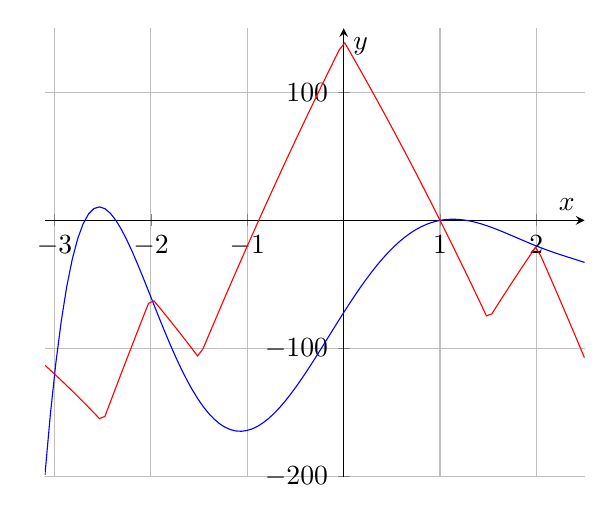
\begin{tikzpicture}[scale=1]
\begin{axis}[
    axis lines = middle,
    grid=major,
    legend pos={south west},
    xlabel = {$x$},
    %xlabel style={below right},
    ylabel = {$y$},
    ymin=-200,
    ymax=150
               ]
	\addplot[domain=-3.1:2.5, samples=100, color=blue] {-(x^2-9)*(x^2-4)*(x-1)*(x-2)+10*x-10*x^2};
\addplot[domain=-3.1:2.5, samples=100, color=red] {70*abs(1-2*abs(abs(x)-2))-10*x^2+10*x-70};
	%\addlegendentry{$\text{Рис. 1}$};
\end{axis}
\end{tikzpicture}\end{center}
